% !TeX root=../main.tex
\chapter{ارائهٔ روش}
\label{proposed}
%\thispagestyle{empty} 
\section{مقدمه} 
روش k-گمنامی اولین بار در مقاله \cite{Sweeney2002} معرفی شده است. با این روش می‌توان اطلاعات مرتبط با افرادی  را که می‌خواهیم گم‌نامی آن‌ها حفظ شود، منتشر نمود. از این روش در سرویس‌های مبتنی بر مکان نیز استفاده می‌شود \cite{Niu2015} . در این سرویس‌ها عموما لازم است کاربر برای دریافت خدمات مرتبط با موقعیت جغرافیایی فعلی خود، اطلاعات مکانی خود را در اختیار ارائه دهنده این خدمات قرار دهد. در  \cite{Niu2015} شرح داده شده است که در صورتی که کاربر اطلاعات مکانی خود را با اطلاعاتی مصنوعی که نشان‌دهنده مکان‌های دیگری هستند ترکیب کند و مجموعه آن‌ها را به سرویس‌دهنده ارسال نماید، می‌تواند تا حدی اطلاعات مکانی خود را پنهان کند. مقاله \cite{Niu2015} با استفاده از معیار آنتروپی توضیح داده که در صورتی که کاربر اطلاعات مصنوعی را به نحوی انتخاب نماید که نرخ (احتمال) پرسمان اطلاعات مربوط به آن مکان‌ها با نرخ پرسمان اطلاعات مکانی خود یکسان باشد، آنتروپی تشخیص مکان کاربر توسط سرویس‌دهنده بیشتر می‌شود. به بیان دیگر سرویس‌دهنده در مورد آن که کدام یکی از موقعیت‌های درخواست داده شده حقیقی و مربوط به کاربر هستند با ابهام بیشتری مواجه خواهد شد.

در این مقاله سعی داریم برخلاف روش مبتنی بر فیلتر بلوم که آدرس‌های مصنوعی به صورت کورکورانه و تصادفی اتخاذ می‌شدند آدرس‌های مصنوعی به نحوی اتخاذ شوند که دارای نرخ پرسمان تقریبا یکسانی با آدرس کاربر درخواست دهنده باشند. در ابتدا تعاریف ریاضی مسئله را بیان کرده و سپس مروری می‌کنیم بر ویژگی‌هایی که لازم است پروتکل ارائه شده از آن‌ها برخوردار باشد.



\subsection{تعریفات ریاضی}




در این مقاله کاربر سبک $i$ام را با $l_i$ نمایش می‌دهیم. مجموعه تمام گره‌های سبک در شبکه به صورت $LW = \{l_1,..., l_M\}$ است که $M$ تعداد کل این گره‌ها است. گره‌ کامل $j$ام به صورت $f_j$ و مجموعه تمام گره‌های کامل به صورت $FN=\{f_1,..., f_W\}$ و تعداد کل گره‌های کامل با $W$ نمایش داده می‌شود. تعداد کل آدرس‌های بیت‌کوین $N$ است و $A=\{a_1,..., a_N\}$ مجموعه تمام آدرس‌ها است. هر آدرس شبکه متعلق به یک گره کامل یا یک گره سبک است. همچنین هر گره می‌تواند مالک چند آدرس باشد. آدرس‌های مربوط به گره سبک $l_i$، که مالک
$C_{l_i}$ 
عدد آدرس است، مجموعه 
$A_{l_i}=\{a_{l_{i1}},... , a_{l_{iC_{l_i}}}\}$
را تشکیل می‌دهد. به همین ترتیب آدرس‌های مربوط به هر کدام از گره‌های کامل تعریف می‌شوند.
%به طوری که:
%\begin{equation}
%	\forall 1<i<M, 1<j<W : A_i, A_j \subset A
%\end{equation}

کاربران سبک اطلاعات جدید مربوط به آدرس‌هایشان را از گره‌های کامل پرسمان می‌کنند. متغیر تصادفی $X_{{a_n}j}$ به این ترتیب تعریف می‌شود که گره کامل $f_j$ آخرین درخواستی که دریافت می‌کند مربوط به آدرس $a_n$ باشد. با توجه به قانون اعداد بزرگ در احتمال، امید ریاضی $X_{{a_n}j}$‌ برابر با تعداد  دفعات درخواست‌های مربوط به آدرس $a_n$ به تعداد کل درخواست‌هایی است که 
$f_j$
، به طوری که
$(1<j<W)$
، دریافت کرده است.
\begin{equation}
E\{X_{{a_n}j}\} = \frac{Q_{{a_n}j}}{Q_{Tj}} \label{eq:1}
\end{equation}
در معامله \eqref{eq:1}،
$E\{X_{{a_n}j}\}$
امید ریاضی پرسمان آدرس $a_n$ از گره کامل
$f_j$ 
است و
$Q_{{a_n}j}$
و
$Q_{Tj}$
به ترتیب تعداد دفعات پرسمان آدرس $a_n$ و تعداد دفعات کل پرسمان‌ها از گره کامل $f_j$ هستند. همچنین می‌توان با استفاده از قانون اعداد بزرگ بورل، احتمال رخداد پیشامد پرسمان $a_n$ در آخرین درخواست انجام شده از گره کامل $f_j$ را برابر امید ریاضی
$E\{X_{{a_n}j}\}$
قرار داد. با توجه به اینکه کاربران سبک در هر نوبت پرسمان به صورت تصادفی یک گره کامل را انتخاب می‌کنند، می‌توان فرض کرد که احتمال پرسمان آدرس‌ها در تمام گره‌های کامل با هم برابر است.
\begin{equation}
Pr\{a_{n}\} = Pr\{a_{nj}\} = E\{X_{{a_n}j}\}, 0<j<M \label{eq:2}
\end{equation}
در معادله \eqref{eq:2}، 
$Pr\{a_{nj}\}$
احتمال پرسمان آدرس $a_n$ از گره کامل
$f_j$ 
است. لازم به ذکر است که احتمال درخواست آدرس‌های مربوط به هر گره‌ کاملی برابر صفر است. چرا که این گره‌ها خودشان وضعیت کامل زنجیره بلوکی را ذخیره کرده‌اند و از گره کامل دیگری در مورد اطلاعات مربوط به آدرس‌هایشان پرسمان انجام نمی‌دهند.
\begin{equation}
Pr\{{a_n}\} = 
\begin{cases}
0, & \text{if}\ a_n \in A_{f_j},\ \ \forall_{j} : 1<j<W \\
Pr\{{a_{l_{ic}}}\}, & \text{if}\ a_n = a_{l_{ic}} \in A_{l_i},\ \ \forall_{i,c} : 1<i<M,\  1<c<C_{l_i}
\end{cases} \label{eq:3}
\end{equation} 

\subsection{ملزومات پروتکل}
\label{subsubsection:4.2}
پیش از پرداختن به ساختار طراحی پروتکل لازم است ویژگی‌هایی که پروتکل باید از آن‌ها برخوردار باشد بررسی شوند. با توجه به هدف پروتکل، که حفظ حریم خصوصی کاربران دارای گره‌های سبک است، لازم است که به مصون ماندن پروتکل نسبت به حملاتی که حریم خصوصی افراد را نقض می‌کنند، توجه ویژه داشت. از طرف دیگر از آن‌جا که کاربران دارای گره‌های سبک امکان پردازش‌ و ذخیره‌سازی حجم بالای اطلاعات را ندارند، همچنین پهنای باند آن‌ها محدود و پر هزینه است، لازم است پروتکل طراحی شده، کمترین میزان بار محاسباتی،‌ مصرف حافظه و پهنای باند را در سمت کاربران سبک داشته باشد. لازم به ذکر است، در صورت وجود فرایند‌های پیچیده در پروتکل، آسیب‌پذیری‌ها و حفره‌های امنیتی زیادی در پروتکل و پیاده‌سازی‌های آن وجود خواهد داشت. از این رو در این پروتکل سعی شده است که تا جای ممکن از فرایند‌های ساده‌ای که پیش از این در کاربرد‌های مختلف آزموده شده‌اند استفاده گردد.

علاوه بر این نباید تغییرات عمده‌ای در ساز و کار گره‌های کامل اعمال کرد و آن‌ها را ملزم به استفاده از ابزارهایی سخت‌افزاری، غیر از سخت افزار مورد نیاز یک گره کامل در شرایط فعلی، نمود. همچنین نباید از نرم‌افزارهایی با مالکیت اختصاصی و متن بسته استفاده شود. این دو کار نه تنها به خاطر دشوار کردن و هزینه‌بر کردن راه‌اندازی یک گره‌کامل، تعداد آن‌ها را در شبکه کمتر می‌کند و منجر به متمرکز شدن شبکه می‌شود، بلکه پروتکل بیت‌کوین را که یک پروتکل بی‌نیاز به اعتماد به یک طرف سوم است، ملزم به اعتماد به شرکت‌های تولید سخت‌افزار‌ و نرم‌افزار‌ به خصوصی می‌کند که وجود درهای پشتی در محصولات آن‌ها اجتناب ناپذیر خواهد بود. 

در ادامهٔ این بخش محدودیت‌ها و  ضوابطی را برای این پروتکل بیان می‌کنیم تا حریم خصوصی کاربر حفظ شده و  همچنین بار محاسباتی، مصرف حافظه و پهنای باند چندانی به طرفین پروتکل اضافه نشود.

نخست، برای آنکه گره کامل $f_j \in FN$ نتواند آدرس $a_{l_{ic}} \in A_{l_i}$ مربوط به گره سبک درخواست دهنده $l_i$ را تشخیص دهد، گره سبک $l_i$ باید اطلاعات مربوط به آدرس خود را به همراه اطلاعت مربوط به $k-1$ عدد از آدرس‌های مصنوعی را همزمان درخواست دهد، به طوری که
$ a_n \in A \textbackslash \{a_{l_{ic}}\}$
. اگر آدرس‌های مصنوعی به نحوی انتخاب شوند که نرخ پرسمان آن‌ها، در زمان درخواست، کمتر از آدرس اصلی باشند، یا اصلا وجود نداشته باشند
($a_n \notin A$)،
گره کامل می‌تواند با احتمال بالاتری آدرس درخواست دهنده را در میان آدرس‌های مصنوعی درخواست داده شده حدس بزند. از این رو باید کاربر سبک آدرس‌های مصنوعی را به نحوی اتخاذ نماید که احتمال درخواست تقریبا برابری با آدرس حقیقی خود داشته باشند، تا گم‌نامی کاربر سبک درخواست دهنده بیشتر حفظ ‌شود. 

دوم، واضح است که محاسبه و پیدا کردن حداقل $k-1$ آدرسی که دارای احتمالی برابر با آدرس کاربر درخواست دهنده باشند، بدون دسترسی به اطلاعات تراکنش‌ها و تناوب درخواست‌ آن‌ها از گره‌های کامل، امری غیر ممکن است. از طرف دیگر اگر کاربر سبک بخواهد این اطلاعات را به طور مستقیم از گره کامل، که دارای تمام این اطلاعات است، دریافت نماید، مشکلاتی اساسی پدید خواهد آمد. در سناریوی پیش رو به دو مورد از آن‌ها اشاره خواهیم نمود.

فرض کنید، $l_i$ در مرحله اول احتمال درخواست آدرس $c$ام خود، یعنی $a_{l_{ic}}$، را حساب نماید. بعدا توضیح داده خواهد شد که این محاسبه بدون نیاز به افشای آدرس به شخص سومی و صرفا بر اساس سوابق کیف پول کاربر قابل انجام است. سپس، احتمال به دست آمده را (بدون ذکر
$a_{l_{ic}}$
) به گره کامل 
$f_{j_1}$
ارسال کرده و  درخواست $k-1$ آدرس با احتمال پرسمان برابر
$Pr\{{a_{l_{ic}}}\}$
بدهد. در مرحله دوم، کاربر آدرس خودش را در میان آدرس‌های مصنوعی هم احتمال قرار داده و اطلاعات مربوط به مجموعه $k$ آدرس حاصل را از یک گره کامل دیگر $f_{j_2}$ یا همان گره کامل پیشین درخواست نماید.  در این سناریو اگر کاربر اطلاعات مجموعه آدرس‌ها را از همان $f_{j_1}$ درخواست نماید، $f_{j_1}$ با توجه به سوابق آدرس‌هایی که قبل‌تر ارسال کرده بوده، متوجه آدرس کاربر، که آدرس جدیدیست و در سوابق اخیرش موجود نیست، می‌شود و آدرس کاربر نزد گره کامل فاش می‌گردد. 

کاربر برای حفظ گم‌نامیش می‌تواند از گره‌ دیگری، مثل $f_{j_2}$ اطلاعات مربوط به مجموعه آدرس‌های هم احتمال را درخواست نماید. در این حالت نیز، در صورتی که $f_{j_1}$ با $f_{j_2}$ تبانی نموده و سوابقشان را با هم به اشتراک بگذارند، طبق روندی که پیش‌تر گفته شد، آدرس فرد درخواست دهنده قابل تشخیص خواهد بود. برای رفع این مشکل کاربر می‌تواند در مرحله اول آدرس‌های هم احتمال را از چند گره متفاوت دریافت نماید و در مرحله دوم زیرمجموعه‌ای تصادفی از تمام آن‌ها را انتخاب و حاصل را به چند بخش تقسیم کرده و هر قسمت را از گره‌ای مجزا درخواست نماید. در این حالت احتمال تشخیص آدرس توسط گره‌هایی که تبانی کرده‌اند کاهش می‌یابد. با این حال، در این روش کاربر سبک باید در صحت هم احتمال بودن آدرس‌های دریافتی به گره‌(ها)ی کامل اعتماد نماید چرا که تصدیق و صحت‌سنجی آن‌ها بدون دسترسی به اصل داده‌ها امکان‌پذیر نیست. به عنوان مثال، در مرحله اول یک گره کامل می‌تواند با ارسال آدرس‌هایی که نرخ پرسمان یکسان، اما متفاوت با نرخ پرسمان آدرس درخواست داده‌شده، داشته باشند، منجر به افشای آدرس کاربر گردد.

از این حیث، لازم است که پروتکل طراحی شده به کاربر سبک اجازه دهد بدون نیاز به فاش کردن اطلاعاتش و همچنین اعتماد به اطلاعات ارسال شده از یک طرف سوم، آدرس‌هایی هم احتمال با آدرس خودش را اتخاذ نموده و مجموعه آن‌ها را از گره کامل پرسمان نماید.

سوم، باید این امر مهم را در نظر بگیریم که کاربران سبک بسیار زیادی هستند که برای به روز رسانی اطلاعاتشان، از طریقی غیر از شبکه‌های حافظ گم‌نامی (مانند تور\RTLfootnote{\lr{Tor}}\cite{torproject}، کراودز\RTLfootnote{\lr{Crowds}}\cite{reiter1998crowds} و غیره)، با گره‌های کامل تبادل اطلاعات انجام می‌دهند. در این صورت مبداء ارسال پرسمان‌های یک کاربر سبک با تقریب خوبی یکسان خواهد ماند. گره کامل متخاصم می‌تواند سابقه‌ای را از پرسمان‌های یک کاربر سبک $l_i$ تشکیل دهد. در این صورت اگر $l_i$ آدرس‌های خودش را، یعنی
$a_{l_{ic}}$
به طوری که
$1<c<C_{l_i}$،
مدام در مجموعه‌ای متفاوت از آدرس‌های هم احتمال قرار دهد، گره متخاصم می‌تواند با اشتراک گیری بین سوابق پرسمان کاربر سبک، به مجموعه‌ای محدودتر از آدرس‌هایی دست پیدا کند که در تمام یا اکثر پرسمانهای آن کاربر وجود داشته‌اند. در نتیجه با احتمال بیشتری می‌تواند آدرس کاربر را تشخیص دهد. برای حفظ گم‌نامی کاربر سبک در برابر این حمله، کاربر سبک باید از مجموعه هم احتمال و تا حد امکان ثابتی استفاده نماید.

در این بخش ملزوماتی برای پروتکل طراحی شده مطرح شدند که علاوه بر آنکه این پروتکل اثر نامطلوبی بر توزیع‌شدگی و امنیت بیت‌کوین نداشته باشد، در برابر حملاتی که ممکن است منجر به فاش شدن آدرس‌های مربوط به یک کاربر سبک گردد مقاوم باشد.

\subsection{ساختار پروتکل}
در این قسمت به توصیف پروتکل پرداخته می‌شود. پروتکل ارائه شده به دو بخش تقسیم می‌گردد. بخش اول شامل فرایندی است که در گره‌های کامل انجام می‌گردد. در این بخش، احتمال پرس‌وجوی تمام آدرس‌های بیت‌کوین ($A$) محاسبه شده و به آدرس‌هایی با احتمال نزدیک به هم تقسیم می‌شوند. به هرکدام از این قسمت‌ها، تکه‌ (Chunk) گفته می‌شود. بخش دوم شامل فرایندی است که گره سبک به صورت آفلاین و بدون نیاز به طرف سومی انجام می‌دهد تا بفهمد که آدرس مربوط به آن در کدام تکه قرار دارد.

در طراحی این پروتکل فرض می‌کنیم که احتمال پرسمان اطلاعات مربوط به هر آدرس $a_n$، به شرطی که مربوط به یک گره کامل نباشد، متناسب است با احتمال استفاده از آن آدرس در شبکه بیت‌کوین. یعنی فرض شده است که هرچه یک کاربر سبک از یک آدرس بیشتر استفاده نماید،‌ بیشتر تمایل دارد اطلاعاتش را در مورد آن آدرس از طریق پرسمان از گره‌های کامل به روزرسانی نماید. به بیان دیگر می‌توانیم بنویسیم:
\begin{equation}
Pr\{{a_n}\} \propto p(a_n) \triangleq \frac{NT_{a_n}}{\sum_{m=1}^{N}NT_{a_m}}; \forall i \  a_n \in A_{l_i}  \label{eq:4}
\end{equation}

در معادله \eqref{eq:4}، 
$NT_{a_n}$
تعداد تراکنش‌هایی هستند که در آن‌ها از آدرس $a_n$ به عنوان ورودی یا خروجی استفاده گردیده و در زنجیره بلوکی بیت‌کوین ثبت شده است. $p(a_n)$ احتمال استفاده از آدرس $a_n$ در شبکه بیت‌کوین تعریف می‌شود. با استفاده از تعریف  \eqref{eq:4} می‌توانیم به تعریفی قابل اجماع از احتمال پرسمان یک آدرس دست پیدا کنیم. دستیابی به این تعریف با توجه به توزیع شدگی و شفافیت و همچنین یکتا بودن وضعیت زنجیره بلوکی در میان تمام گره‌های شبکه قابل انجام است.  

\subsubsection{محاسبه مستقل از دیگر آدرس‌ها}
\label{subsubsection:4.3.1}
کاربران سبک  باید بتوانند بدون نیاز به هر درخواست اطلاعات اضافه‌ای از گره کامل، محاسبه نمایند که آدرس‌های آن‌ها در کدام تکه قرار گرفته است. فرایند انجام این محاسبه به طور کامل در بخش \ref{subsubsection:4.3.3} توضیح داده شده است. در این بخش می‌خواهیم پروتکل را به نحوی طراحی کنیم که گره‌های سبک بدون نیاز به پرسیدن چیزی از گره دیگری، بتوانند تکه مربوط به خود را مشخص نماید. در گام اول لازم است به این موضوع اشاره شود که گره‌های سبک امکان محاسبه $NT_{a_n}$ مربوط به آدرس خود را به صورت آفلاین و با توجه به سوابق تراکنش‌هایشان دارند. به خاطر یکسان بودن
$\sum_{m=1}^{N}NT_{a_m}$
نیازی نیست که کاربران سبک از آن اطلاع داشته باشند.

مسئله دیگری که لازم است مورد توجه قرار گیرد، ارائه روشی برای محاسبه آدرس‌های هر تکه به صورتی است که نه تنها با تغییر عمده نرخ پرسمان یک آدرس، آدرس در تکه‌ای جدا و متناسب با نرخ جدید قرار بگیرد و در تکه قبلی نماند، بلکه با توجه به آنچه در بخش \ref{subsubsection:4.2} بحث شده بود، لازم است که تکه‌ها نسبت که تغییرات اندک نرخ پرسمان آدرس‌ها مقاوم باشند. تغییر خیلی کند تکه‌ها باعث می‌شود که آنتروپی هر تکه کاسته شود و از طرف دیگر تغییر سریع تکه‌ها باعث می‌شود که گره کامل با اشتراک گیری درخواست‌هایی که از یک منبع ثابت ارسال می‌شوند، به تعداد محدودتری از آدرس‌های محتمل برای گره سبک درخواست دهنده دست یابد.

برای رسیدن به این هدف ابتدا تعریفی از امتیاز هر آدرس در زمان $t_0$ به صورت 
$s_{a_n}^{t_0}$
تعریف می‌کنیم. مجموعه تمام این امتیاز‌ها در یک زمان خاص، حالت سیستم در آن زمان نامیده می‌گردد. 
\begin{equation}
\forall\ a_n\ \text{in}\  A\  \text{at}\  t_0: S^{t_0} = [s_{a_1}^{t_0}, ..., s_{a_n}^{t_0}]^T  
\label{eq:5}
\end{equation}
که
$S^{t_0}$
حالت سیستم در پنجره زمانی $t_0$ است. پنجره زمانی با $W$ مشخص شده و به این صورت تعریف می‌شود: پارامتر $W$ برابر با تعداد بلوک‌هایی است که نشان‌دهنده یک واحد زمانی هستند. بعد از استخراج $W$ بلوک و ثبت آن در زنجیره بلوکی بیت‌کوین، حالت سیستم با توجه به $W$ بلوک اخیر استخراج شده به روزرسانی می‌گردد. به این ترتیب امتیاز آدرس $a_n$ در پنجره زمانی  $t_0$  ($W^{t_0}$)به صورت $s_{a_n}^{t_0}$ نمایش داده شده و به صورت معادله \eqref{eq:6} تعریف می‌شود.
\begin{equation}
s_{a_n}^{t_0} = \beta NT_{a_n}^{t_0} + (1-\beta) s_{a_n}^{t_{-1}}
\label{eq:6}
\end{equation}

که
$0<\beta<1$
و
$NT_{a_n}^{t_0}$
تعداد تراکنش‌هایی است که شامل آدرس $a_n$ در ورودی یا خروجیشان بوده‌اند و در بلوک‌های موجود در پنجره زمانی $W^{t_0}$ ظاهر شده‌اند است. به این ترتیب حالت کلی سیستم ($S^{t_0}$ ) به صورت معادله \eqref{eq:7} به روزرسانی می‌شود.
\begin{equation}
S^{t_0} = \beta NT_{A}^{t_0} + (1-\beta) S^{t_{-1}}
\label{eq:7}
\end{equation}
که 
$NT_{A}^{t_0} = [NT_{a_1}^{t_0}, ..., NT_{a_N}^{t_0}]^T$
است. به این ترتیب توانستیم امتیاز هر کدام از آدرس‌ها را مستقل از آدرس‌های دیگر محاسبه نموده و با تنظیم پارامتر $\beta$ و اندازه $W$ سرعت تغییرات تکه‌ها را تنظیم نماییم. اندازه پنجره‌های زمانی نیز بر اساس تعداد بلوک‌های استخراج شده تعیین می‌شوند. به خاطر آنکه زمان بین استخراج دو بلوک تقریبا زمان ثابتی و برابر با ۱۰ دقیقه فرض می‌شود، زمان به روزرسانی امتیاز هر کدام از آدرس‌ها تقریبا ثابت خواهد بود. به عنوان مثال اگر اندازه پنجره زمانی ۱۴۴ بلوک در نظر گرفته شود، تقریبا هر ۲۴ ساعت یک بار امتیاز آدرس‌ها به روز رسانی می‌گردد.  


\subsubsection{تعیین و انتشار تکه‌ها}
\label{subsubsection:4.3.2}
در قسمت قبل، برای هر آدرس امتیازی در نظر گرفته شد و توضیح داده شد که چطور در هر پنجره زمانی وضعیت امتیاز تمام آدرس‌ها به روز رسانی می‌گردد. در این بخش با توجه به چگونگی توزیع امتیاز آدرس‌ها، که در شکل \ref{fig:log2scale} قابل مشاهده است، مرز بین تکه‌ها و تعداد اعضا هر تکه را به نحوی انتخاب می‌کنیم که نه تنها باعث کاهش امنیت و گم‌نامی گره‌های سبک نگردد، بلکه پهنای باند مصرف شده جهت پرسمان تمام آدرس‌های یک تکه مقرون به صرفه باشد.

با توجه به معادله \eqref{eq:3} احتمال پرسمان آدرس $a_n$ به شرطی که برای یک گره کامل نباشد برابر $Pr\{{a_n}\}$ و مخالف صفر است. اگر گره سبک $l_i$ بخواهد اطلاعات مربوط به آدرس $a_{l_{ic}}$ را که مربوط به خودش است درخواست نماید لازم است اطلاعات مربوط به آدرس‌های هم احتمال با خودش را که یک تکه‌ را تشکیل می‌دهند (مثلا تکه شماره $\gamma$) دریافت نماید. تعداد اعضای این تکه را با $K_\gamma$ نمایش می‌دهیم. از منظر گره کامل هر کدام از $K_\gamma$  آدرس‌ موجود در تکه درخواست داده شده ممکن است برای درخواست دهنده ($a_{l_{ic}}$ ) باشد. احتمال آنکه هر کدام از آدرس‌های تکه، آدرس مورد نظر باشد را با $q_k$ نشان می‌دهیم که $k=(1, 2, ..., K_\gamma)$. به این ترتیب $q_k$ به صورت زیر تعریف می‌شود.

\begin{equation}
q_k = \frac{Pr\{a_{\gamma k}\}}{\sum_{m=1}^{K_\gamma}Pr\{a_{\gamma m}\}}; \quad \sum_{k=1}^{K_\gamma} q_k = 1
\label{eq:8}
\end{equation}

که $Pr\{a_{\gamma m}\}$ احتمال پرسمان آدرس $k$ام مربوط به تکه‌ $\gamma$ است. به این ترتیب آنتروپی تشخیص آدرس مورد نظر از میان آدرس‌های تکه $\gamma$ به صورت معادله \eqref{eq:9} قابل محاسبه خواهد بود:
\begin{equation}
H = -\sum_{k=1}^{K_\gamma} q_k . \log_2 q_k
\label{eq:9}
\end{equation}

که هر چه آنتروپی ($H$) بزرگ‌تر باشد به معنی حفظ بیشتر گم‌نامی آدرس مورد نظر است است. زمانی این مقدار ماکزیمم است که تمام $K_\gamma$ عضو تکه، احتمالی برابر داشته باشند. این مقدار ماکزیمم برابر $H_{max} = \log_2K_\gamma$ است.

با فرض اینکه احتمال پرسمان یک آدرس مربوط به گره سبک متناسب است با احتمال قرارگیری این آدرس در تراکنش‌های موجود در زنجیره بلوکی بیت‌کوین (معادله \eqref{eq:4}) می‌توانیم برای تعیین  تکه‌ها و ساخت آن‌ها با توجه به امتیاز آدرس‌ها (فرمول \eqref{eq:5}) عمل نماییم. جهت نحوه مرزبندی تکه‌ها لازم است به نکات زیر توجه شود:

\begin{enumerate}
	\item{%
		هرچه مقدار $K_\gamma$ برای تکه $\gamma$ بیش‌تر باشد، آنتروپی آن بیشتر خواهد بود. بالا رفتن $K_\gamma$ باعث می‌شود که کاربر سبک به ازای هر درخواست، اطلاعات اضافه بیشتری را دریافت نماید. در نتیجه پهنای باند و ترافیک زیادی مصرف نماید. 	
	}
	\item{%
		با توجه به شکل \ref{fig:log2scale} مشاهده می‌شود که اکثر آدرس‌های استفاده شده در بیت‌کوین دارای امتیازی کمتر از یک هستند و آدرس‌هایی که امتیاز آن‌ها بیشتر از یک است بسیار کم و پراکنده هستند. از این رو اگر مرز بین تکه‌‌ها به صورت توان‌های دو
		$(..., 2^{-2}, 2^{-1}, 2^{0}, 2^{1}, 2^{2},...)$
		انتخاب شوند، در آدرس‌هایی با امتیاز کمتر از ۱، مقدار آدرس‌های تقریبا یکسانی در هر تکه قرار خواهند گرفت.
	}
	\item{%
		این شیوه قسمت‌بندی، امنیت و گم‌نامی زیادی برای آدرس‌های پر استفاده ایجاد نمی‌کند. زیرا اولا، تعداد اعضای تکه‌های آدرس‌های پر استفاده کمتر است. ثانیا، مرز این تکه‌ها گستره‌تر بوده که باعث می‌شود که آدرس‌هایی با رنج وسیعی از احتمال پرسمان را در خود جایی دهد. با این حال می‌توان استدلال کرد که آدرس‌های پر استفاده، به منظور حفظ بیشتر امنیت، مربوط به گره‌های کامل هستند یا اینکه بهتر است دارندگان این آدرس‌ها به جای استفاده از یک گره سبک،  یک گره کامل راه‌اندازی نمایند. 
	}
	\item{%
		با توجه به اینکه تکه‌های مربوط به آدرس‌های کم استفاده (با امتیاز کمتر از ۱) تعداد اعضای زیادی خواهند داشت و بارگیری آن‌ها توسط گره سبک مصرف زیاد پهنای باند و ترافیک شبکه را به همراه خواهد داشت، می‌توان از دو رویه برای آن‌ها استفاده نمود. یک، از توان‌های اعشاری برای جداسازی تکه‌های آدرس‌های کم‌ استفاده بهره برد. دو، آدرس‌های مربوط به یک تکه با اعضای زیاد را به ترتیب الفبا مرتب نمود و با توجه به حروف الفبا آن‌ها را تقسیم بندی نمود. به عنوان مثال آدرس‌هایی مربوط به یک تکه که با
		\lr{bc1qaaa}
		آغاز می‌شوند درون یک زیر تکه قرار بگیرند و آدرس‌هایی که با \lr{bc1qaac} شروع می‌شوند در یک زیر تکه دیگر قرار گیرند (در استاندارد آدرس بک-۳۲ \RTLfootnote{\lr{Bech-32}} از کاراکتر b استفاده نمی‌شود \cite{Wuille2017}). روش دوم از روش اول برتری دارد. از آن جهت که در روش اول تغییرات تکه‌ها افزوده خواهد شد. در بخش \ref{subsubsection:4.2} توضیح داده شد که تغییرات زیاد تکه‌ها باعث کاهش گم‌نامی خواهد شد.
	}
	
\end{enumerate}
در این بخش به شیوه بهینه تشکیل تکه‌ها و اهمیتی که بر حفظ گم‌نامی کاربران سبک ایفا می‌کند پرداخته شد. تکه‌های تشکیل شده در این روش در تمام شبکه، که یک زنجیره بلوکی واحد را به اشتراک می‌گذارند، یکتا است. به این ترتیب هر آدرس  در زمان $t_0$ تنها در یک تکه به خصوص قرار خواهد داشت. تشخیص این که گره کاربر سبک در کدام تکه قرار دارد، به صورت آفلاین و بدون نیاز به درخواست اطلاعات اضافه‌ای، توسط خود کاربر قابل انجام است. از این رو،‌ کاربر می‌تواند تنها با ارسال شماره تکه ($\gamma$) و زیرتکه (جداسازی الفبایی) به صورت امن به اطلاعات مربوط به آدرس خودش دست پیدا کند.


\begin{figure}[t]
	\centering
	\includegraphics[width=0.7\linewidth]{/home/taghi/Projects/Bitcoin_Address_Extractor/Analysis/Log2_scale}
	\caption[امتیاز آدرس‌های بیت‌کوین در مقیاس لگاریتمی]{امتیاز آدرس‌های بیت‌کوین در مقیاس لگاریتمی از تاریخ ۲۶ ژوئن ۲۰۱۹ الی ۰۲ دسامبر ۲۰۱۹}
	\label{fig:log2scale}
\end{figure}


\subsubsection{محاسبه آفلاین در سمت کاربر سبک}
\label{subsubsection:4.3.3}
تا اینجا، نحوه تکه‌بندی آدرس‌ها با توجه به امتیاز هر آدرس، که مطابق معادله \eqref{eq:6} محاسبه گردید، توضیح داده شد. طراحی پروتکل به نحوی انجام شد که کاربران سبک بتوانند بدون نیاز به ارسال هیچ اطلاعات اضافه‌ای، از تکه‌ای که مربوط به خودشان است آگاه شوند. از این رو محاسبه آفلاین تکه در سمت کاربر به امری ساده تبدیل شد. در این بخش به نحوه انجام این محاسبه خواهیم پرداخت.

کاربر سبک همگام با شبکه، سرایند تمام بلوک‌های زنجیره بلوکی را دارد و همچنین می‌داند که تمام تراکنش‌هایی که در آن‌ها از آدرس وی استفاده شده است، در کدام بلوک‌ها قرار دارند. از این رو کاربر سبک می‌تواند به راحتی با توجه به سوابقی که در اختیار دارد و با استفاده از فرمول \eqref{eq:6} از شماره تکه‌ای که شامل آدرس خودش است مطلع شود. کاربر سبک همچنین می‌تواند به راحتی تشخیص دهد که آدرسش، با توجه به تقسیم‌بندی الفبایی، در کدام زیر تکه قرار دارد. 

اگر کاربر سبک تمام سوابق خودش را از دست دهد، می‌تواند زیر تکه متناسب با آدرسش را از تمام تکه‌های موجود درخواست دهد. استفاده از روش چینش الفبایی کمک می‌کند که کاربر سبک  زیرتکه‌های کمتری را امتحان کرده و درنتیحه ترافیک شبکه کمتری مصرف نماید.

از آن‌جایی که محاسبهٔ امتیاز هر آدرس با توجه به زنجیره بلوکی تعیین می‌شود، مقدار آن قابل اجماع است. از این رو گره‌های کامل می‌توانند به صورت روزانه (به ازای هر $144$ بلوک) امتیازها را بروز رسانی نموده و لیست آدرس‌های جدید همراه با امتیاز آن‌ها را در شبکه قرار دهند. همچنین، می‌توان درخت مرکل تمام آدرس‌ها را تولید کرده و در تراکنش کوین‌بیس قرار دهند. به این ترتیب گره سبکی که تاریخچه اطلاعاتش را از دست داده می‌تواند ساده‌تر به دنبال آدرس خودش بگردد و از صحت امتیاز آدرسش مطمئن شود.


%{\color{red}در قالب یک بلوک الگوریتم تمام کار‌هایی که باید انجام دهد نوشته شود.
%	
%	\color{red}امکان اضافه کردن PIR سنجیده شود.
%	
%	\color{red} زمان و پهنای باند querry ها سنجیده شود.
%	
%	\color{red} به نظر می‌رسد که بررسی تنها آدرس‌هایی که موجودی غیر صفر دارند کافی باشد.
%	
%}

\subsubsection{پیاده‌سازی و شبیه‌سازی}
\label{subsubsection:4.3.4}


در پیاده‌سازی انجام شده \cite{Badakhshan}، از پایگاه‌دادهٔ 
ردیس\RTLfootnote{Redis}
برای ذخیره‌سازی وضعیت هر آدرس و امتیاز آن استفاده شده است. شبیه‌سازی پروتکل مستقیما بر روی دادگان خام زنجیره بلوکی بیت‌کوین انجام گرفته. این شبیه‌سازی بر روی دادگان از تاریخ ۲۶ ژوئن ۲۰۱۹ الی ۰۲ دسامبر ۲۰۱۹ صورت گرفت. در این بخش به بررسی این نتایج خواهیم پرداخت. برای نشان‌دادن بهتر وضعیت آدرس‌ها،  تعداد تکه‌ها زیاد‌تر انتخاب شده است به این ترتیب که بازهٔ آن‌ها به صورت
$\{(0,2^{-20}), (2^{-20}, 2^{-19}), (2^{-19}, 2^{-18}), ..., (2^{20}, \infty)\}$ 
است.

پیاده‌سازی به این صورت است که به ازای هر روز، آدرس‌های موجود در تمام بلوک‌های استخراج شده در آن روز به همراه امتیاز آن ذخیره می‌شود و با توجه به این امتیاز‌ها و وضعیت قبلی ($S^{t_{-1}}$)، وضعیت جدید محاسبه می‌شود.

یکی از اصلی‌ترین معیار‌های سنجش عملکرد صحیح پروتکل عدم تغییر سریع آدرس‌ها در میان تکه‌های مختلف است. با تنظیم پارامتر $\beta$، که در معادله \eqref{eq:6} تعریف شد، و همچین بازه‌ی تکه‌ها می‌توان سرعت تغییر آدرس‌ها در میان تکه‌ها را کنترل نمود. همان‌طور که در شکل \ref{fig:changed} نمایش داده شده است، تغییرات کلی آدرس‌ها، به ازای $\beta=0.3$، در حول مقدار ثابتی نوسان می‌کند.

\begin{figure}[h]
	\centering
	\includegraphics[width=0.7\linewidth]{/home/taghi/Projects/Bitcoin_Address_Extractor/Analysis/changed}
	\caption{%
		نمودار جابه‌جایی آدرس‌ها در میان تکه‌های مختلف از تاریخ ۲۶ ژوئن ۲۰۱۹ الی ۰۲ دسامبر ۲۰۱۹. ($\beta=0.3$)
	}
	\label{fig:changed}
\end{figure}

زمان مصرف شده به ازای به روزرسانی روزانهٔ آدرس‌ها در شکل \ref{fig:time_proposed} نمایش داده شده است. همان‌طور که مشاهده می‌شود، این روش سربار پردازشی زیادی بر روی گره‌های کامل اعمال نمی‌کند.

\begin{figure}
	\centering
	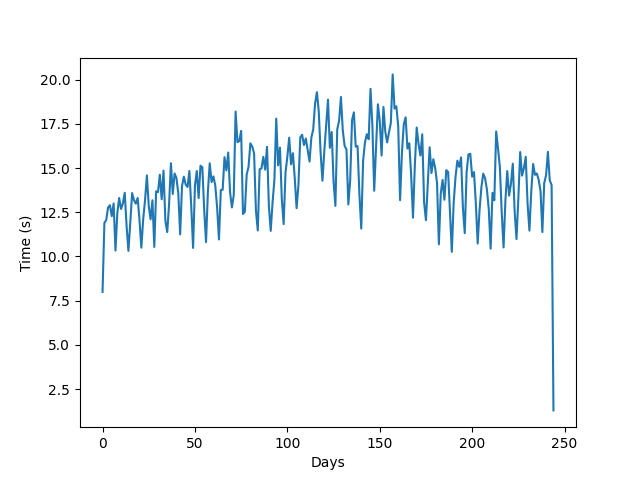
\includegraphics[width=0.7\linewidth]{image/time}
	\caption{زمان‌ به روز رسانی وضعیت امتیاز‌ها برای هر روز}
	\label{fig:time_proposed}
\end{figure}

شکل \ref{fig:betachange} درصد تغییرات آدرس‌ها در بین تکه‌های مختلف نسبت به کل آدرس‌ها با توجه به مقدرا $\beta$ را نشان می‌دهد. هر چه این مقدار به $1$ نزدیک  تر باشد، امتیاز آدرس‌ها سریع‌تر تغییر می‌کند.

\begin{figure}
	\centering
	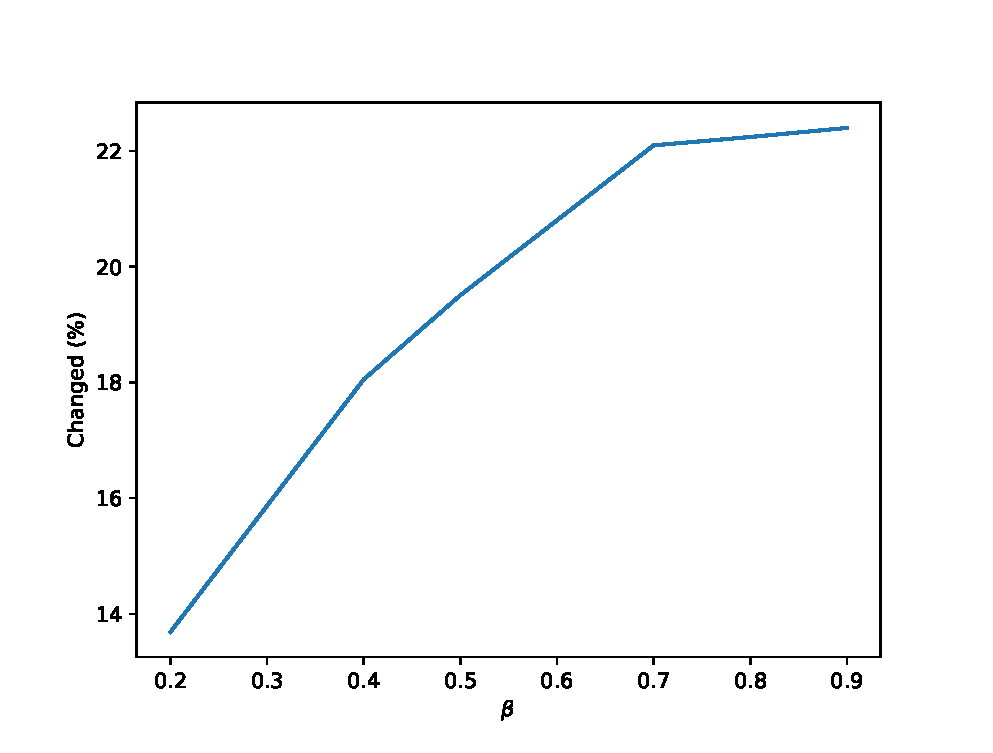
\includegraphics[width=0.7\linewidth]{image/beta_change}
	\caption{درصد آدرس‌های تغییر کرده در بین تکه‌های مختلف به تعداد کل آدرس‌ها با توجه به اندازهٔ $\beta$}
	\label{fig:betachange}
\end{figure}



\subsubsection{بحث و نتیجه‌گیری}

در روش ارائه شده سعی شده است که بدون نیاز به استفاده از پروتکل و ابزار‌های پیچیده، با حذف فیلتر بلوم بهره‌گیری از معیار ‌$K$-گمنامی و قرار دادن آدرس‌هایی با احتمال درخواست یکسان، در یک دسته به سطح بالاتری از امنیت نسبت به فیلتر بلوم دست پیدا شود. همچنین در این روش تعیین پهنای باند مصرفی کاملا در اختیار کاربر سبک است و کاربر سبک می‌تواند با سطح امنیت مورد نظرش این مقدار را تعیین کند.

مقدار $\beta$ باید پیش از راه‌اندازی پروتکل تعیین شود. هر چه این مقدار بیش‌تر باشد، تغییرات آدرس‌ها در تکه‌ها سریع‌تر بوده و به گره کامل متخاصم امکان می‌دهد که با اشتراک‌گیری، آدرس مورد نظر کاربر را تشخیص دهد، از طرف دیگر اگر مقدار آن کم باشد باعث می‌شود که آدرس‌هایی که در یک تکه قرار گرفته‌اند در حال حاضر مقدار امتیاز مشابهی نداشته باشند در نتیجه، طبق فرمول \eqref{eq:9} آنتروپی آدرس‌ها در یک تکه کاهش پیدا می‌کند. در نتیجه باید بررسی‌های بیش‌تری برای انتخاب $\beta$ انجام گیرد.

\begin{xltabular}{\textwidth}{|r|X|}
	\caption{
		مقایسهٔ  امنیت، پهنای باند و پردازش سمت گره کامل برای روش ارائه شده
		\label{table:Proposed}}\\
	\hline
	\textbf{معیار} & \textbf{توضیحات} \\
	\hline
	{%
		امنیت
	}&{%
		امکان تعیین آدرس‌های پوششی به صورت هوشمندانه و به مقدار دلخواه، استقلال بین درخواست‌های کاربر و دشواری ایجاد پیوند بین درخواست‌های وی، مقاوم در برابر تحلیل بسامد استفاده از آدرس، عدم نیاز به تجهیزات سخت‌افزاری و نرم‌افزاری پیچیده و امکان راه‌اندازی ساده‌ٔ یک گره کامل و در نتیجه کاهش نیاز به اعتماد به گره‌های محدود جهت دریافت خدمات
	}\\
	\hline
	{%
		پهنای باند مصرفی
	}&{%
		پهنای باند مصرفی قابل تنظیم که تنها شامل تراکنش‌های اصلی به علاوه تراکنش‌های پوششی و اثبات مرکل آن‌ها است.
	}\\
	\hline
	{%
		پردازش سمت کاربر کامل
	} & {%
	با توجه به شکل \ref{fig:time_proposed} به ازای به روز رسانی هر روزانه، زمان زیادی صرف نمی‌شود.
}\\
\hline
\end{xltabular}





